\subsection{Eigenschaften}

Die \textit{Characteristics} umfassen jene Eigenschaften von Erklärungen, die einen Einfluss auf die externe Qualität eben dieser haben. Unter dem Aspekt sind die Möglichkeiten zusammengefasst, die bei der Ausgestaltung von Erklärungen bestehen. Gegliedert sind die Eigenschaften in den Bedarf der Erklärung (\textit{Demand}), die ausgelieferten Informationen (\textit{Content}) und die Bereitstellung (\textit{Presentation}). Diese drei Unterkategorien werden in den folgenden Abschnitten vorgestellt. Die vorangegangenen Arbeiten, in denen einzelne Eigenschaften untersucht wurden, werden in diesem Abschnitt jeweils in eigenen Tabellen mit aufgeführt, um als Beispiele für diese zu dienen. Wichtig zu beachten ist, dass sich die vorgestellten Möglichkeiten nicht unbedingt ausschließen. Das heißt vor allem, dass nicht jede Erklärung genau eine Ausprägung eines Aspektes erfüllen muss, sondern auch neue oder zwischen zwei Möglichkeiten liegende Eigenschaften aufweisen kann. Darüber hinaus muss auch nicht zwangsweise für jede Eigenschaftskategorie eine Eigenschaft ausgewählt werden, da nicht alle Kategorien auf jeden Kontext zutreffen.

\begin{figure}[htb!]
    \begin{center}
        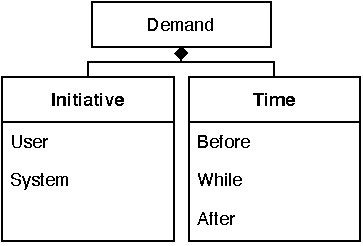
\includegraphics{contents/05_model_description/res/model_demand_overview.pdf}
    \end{center}
    \caption{Übersicht über den \textit{Demand} für Erklärungen}
    \label{fig:model_demand_overview}
\end{figure}

\subsubsection{Bedarf}

Der \textit{Demand}  für Erklärungen kann aus verschiedenen Perspektiven betrachtet werden. Bei welcher Aufgabe und bei welchen Ereignissen Erklärungen überhaupt benötigt werden, muss in den Anforderungen für Erklärungen festgehalten werden. Diese entstehen auf Basis der \textit{External Dependencies}. Unter der Kategorie \textit{Demand} in diesem Modell ist zusätzlich festgehalten, mit welcher Initiative (\textit{Initiative}) und wann genau in Bezug auf ein Ereignis im System dem \textit{End User} Erklärungen vom System zur Verfügung gestellt werden sollen. Einen Überblick über die Verwendung verschiedener Ausprägungen der Aspekte ist in \autoref{fig:model_demand_overview} und \autoref{tab:explanation_demands} dargestellt.

\begin{table}[bht!]
    \begin{center}
        \begin{tabular}{p{.25\textwidth}p{.25\textwidth}p{.41\textwidth}}
            \hline
            Aspekt    & Ausprägung   & Quellen \\
            \toprule
            initiative  &  Manual       & \cite{chazette_end-users_nodate} \cite{tintarev_designing_nodate}
                                            \cite{wiegand_id_2020} \\
                        &  Automatic    & \cite{chazette_end-users_nodate} \cite{eiband_impact_2019}
                                            \cite{wiegand_id_2020} \cite{schaffer_i_2019}
                                            \cite{yamada_evaluating_2016} \\
            \tablerowspacing
            Time        &  Before       & \cite{rosenfeld_explainability_2019} \cite{wiegand_id_2020}
                                            \cite{kunkel_let_2019} \cite{koo_why_2015} \cite{haspiel_explanations_2018} 
                                            \cite{haspiel_explanations_2018} \\
                        &  while        & \cite{rosenfeld_explainability_2019} \cite{wiegand_id_2020}
                                            \cite{kunkel_let_2019} \\
                        &  After        & \cite{rosenfeld_explainability_2019} \cite{wiegand_id_2020}
                                            \cite{kunkel_let_2019} \cite{koo_why_2015} \cite{haspiel_explanations_2018}
                                            \cite{wiegand2019drive} \cite{haspiel_explanations_2018} \\
            \toprule
        \end{tabular}
    \end{center}
    \caption{Der Bedarf einer Erklärung zusammen mit in der Literatur untersuchten Einflüssen auf die Qualität von Erklärungen}
    \label{tab:explanation_demands}
\end{table}

\paragraph{Initiative} Die \textit{Initiative} einer Erklärung ist der Auslöser für das Geben von Erklärungen in einem System. Eine Möglichkeit ist eine automatische Auslieferung der Erklärung an den \textit{End User}. Das System trifft dann allein die Entscheidung, wann und ob \textit{End User} eine Erklärung bekommt (\textit{Automatic}). Alternativ können Erklärungen vom \textit{End User} manuell angefordert werden (\textit{Manual}). Auch Mischformen, bei der \textit{End User} beispielsweise festlegen können, welche Art von Erklärungen sie erhalten möchten, sind denkbar.

\paragraph{Time} Die \textit{Time} ist der Zeitpunkt im Verhältnis zu einem Ereignis, zu dem das System eine Erklärung bereitstellt. \citeauthor{rosenfeld_explainability_2019} sowie \citeauthor{wiegand_id_2020} haben explizit untersucht, wann Erklärungen angezeigt werden sollten, wenn ein Ereignis im System auftritt oder das System eine Aktion durchführt. Dies umfasst die Möglichkeiten vor dem Ereignis (\textit{Before}), während (\textit{While}) oder nach dem Ereignis (\textit{After}) eine Erklärung zu diesem zu liefern \cite{rosenfeld_explainability_2019, wiegand_id_2020}. Letzteres wird in der Literatur zum Teil auch als \textit{Posthoc-Explanation} referenziert \cite{sokol_explainability_2020}.

\smallskip

Im Rahmen von \textbf{RQ2} kann an dieser Stelle folglich abgeleitet werden, dass der \textit{Demand} mit den verschiedenen Möglichkeiten für \textit{End User} eine Erklärung zu bestimmten Zeitpunkten zu erhalten eine Eigenschaft mit einem Einfluss auf die externe Erklärungsqualität ist.

\begin{figure}[htb!]
    \begin{center}
        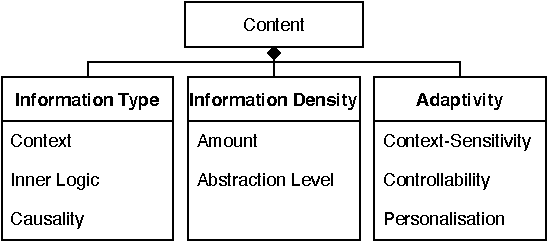
\includegraphics{contents/05_model_description/res/model_content_overview.pdf}
    \end{center}
    \caption{Übersicht über den \textit{Content} von Erklärungen}
    \label{fig:model_content_overview}
\end{figure}

\subsubsection{Inhalt}

Unter dem Punkt \textit{Content} wird definiert, mit welchen Inhalten die \textit{End User} durch Erklärungen versorgt werden \cite{nunes_systematic_2017}. Dieser ist einer von zwei Teilen des Modells, welcher sich auf die Granularität von Erklärungen bezieht. Der \textit{Content} beinhaltet nicht nur den Informationstyp (\textit{Information Type}) den das System vermittelt, sondern auch wie viel Inhalt (\textit{Information Density}). Ein weiterer Aspekt ist Anpassungsfähigkeit der Inhalte (\textit{Adaptivity}). \autoref{tab:content_of_explanations} und \autoref{fig:model_content_overview} enthalten die verschiedenen Ausprägungen dieser Aspekte zusammen mit deren Anwendungen in der Literatur, welche einen Einfluss auf die externe Qualität von Erklärungen haben.

\begin{table}[bht!]
    \begin{center}
        \begin{tabular}{p{.25\textwidth}p{.25\textwidth}p{.41\textwidth}}
            \hline
            Aspekt    & Ausprägung   & Quellen \\
            \toprule
            Information Type        & Context     & \cite{chazette2020explainability} \cite{zahedi_towards_2019}
                                                \cite{cassens_ambient_2019} \cite{zahedi_towards_2019}
                                                \cite{zolotas_towards_2019} \cite{chari_explanation_2020}
                                                \cite{nunes_systematic_2017} \cite{ribera2019can} \\
                            & Inner Logic & \cite{chazette2020explainability} \cite{sato_action-triggering_2019} 
                                                \cite{thomson_knowledge--information_2020}
                                                \cite{chari_explanation_2020} \cite{neerincx_using_2018}
                                                \cite{ribera2019can} \cite{cassens_ambient_2019} \\
                                & Causality &   \cite{chazette2020explainability} \cite{abdulrahman_belief-based_2019}
                                                \cite{yamada_evaluating_2016} \cite{sato_action-triggering_2019}
                                                \cite{zahedi_towards_2019} \cite{zahedi_towards_2019}
                                                \cite{zolotas_towards_2019} \cite{cassens_ambient_2019}
                                                \cite{thomson_knowledge--information_2020}
                                                \cite{chari_explanation_2020} \cite{neerincx_using_2018}
                                                \cite{nunes_systematic_2017}\cite{zhu_effects_2020}
                                                \cite{ribera2019can} \cite{lim_2009_assessing} 
                                                \cite{kaptein_personalised_2017} \\
            \tablerowspacing
            Information          & Amount &      \cite{ribera2019can} \cite{kouki_user_2017}
                                                \cite{hernandez-bocanegra_effects_2020} \cite{martin_developing_2019} \\
            Density              & Abstraction Level & \cite{thomson_knowledge--information_2020}
                                                \cite{hernandez-bocanegra_effects_2020} \\
            \tablerowspacing
            Adaptivity          & Context-Sensitivity & \cite{kaptein_personalised_2017} \cite{cassens_ambient_2019} \\
                                & Controllability & \cite{abdulrahman_belief-based_2019} \cite{cheng2019explaining} \\
                                & Personalization & \cite{kaptein_personalised_2017} \cite{cassens_ambient_2019}
                                                    \cite{sokol_one_2020} \cite{tintarev_designing_nodate}
                                                    \cite{sokol_explainability_2020} \\
            \toprule
        \end{tabular}
    \end{center}
    \caption{Eigenschaften einer Erklärung bezogen auf den Inhalt einer Erklärung mit in der Literatur gezeigtem Einfluss auf die externe Qualität von Erklärungen}
    \label{tab:content_of_explanations}
\end{table}

\paragraph{Information Type} Der \textit{Information Type} beschreibt die Inhalte, die \textit{End Usern} mithilfe der Erklärung übermittelt werden. Unter diesem Aspekt sind in der Literatur sehr verschiedene Ansätze zu finden, die unterschiedliche Typen definieren. Beispielsweise stellen \citeauthor{chazette_end-users_nodate} mithilfe von Fragewörtern verschiedene Informationstypen dar \cite{chazette_end-users_nodate}, während \citeauthor{rosenfeld_explainability_2019} selbige Fragewörter nutzt, um andere Inhalte zu beschreiben und weitere ergänzt. Grundsätzlich kann zwischen globalen Erklärungen, die immer gültig sind und situationsabhängigen (lokalen) Erklärungen unterschieden werden \cite{lim_2009_assessing}. Zusammen mit weiteren \cite{kaptein_personalised_2017, abdulrahman_belief-based_2019} wurden die verschiedenen Definitionen in drei verschiedene Informationstypen gebündelt.

Kontextinformationen in einer Erklärung geben Auskunft über die zugrundeliegenden Daten (\textit{Context}). Dabei werden die eingehenden Informationen auf Basis derer das System Entscheidungen trifft, dem \textit{End User} dargelegt.

Eine weitere Möglichkeit ist das Erklären der Funktionsweise von Algorithmen eines Systems (\textit{Inner Logic}). Dies enthält die Informationen, wie genau ein System die ihm zur Verfügung stehenden Informationen verarbeitet und interpretiert.

Ein dritter Weg ist die Erklärung von Zusammenhängen zwischen den Eingaben und Ausgaben des Systems (\textit{Causality}). In einer solchen Erklärung wird den \textit{End Usern} der Grund für ein bestimmtes Systemverhalten oder eine Entscheidung erläutert. Dieser Punkt lässt sich in weitere Möglichkeiten gliedern, Gründe zu erläutern. Eine Erklärung dieser Art kann die Information enthalten, warum ein bestimmtes Systemverhalten in einer Situation erfolgt ist. Auch kann eine Erklärung klarstellen, warum ein alternatives Verhalten oder eine alternative Ausgabe des Systems nicht erfolgt ist \cite{martin_evaluating_2021}. % \cite{lim_2009_assessing} sagt, dass counterfactual nicht trivial ist.

% the different types of content answer the gulfs of execution and evaluation of \cite{norman1988psychology} as described by \cite{ribera2019can}

\paragraph{Information Density} Die \textit{Information Density} beschreibt die Menge und die Kompaktheit an Informationen die eine Erklärung enthält. Dabei ist einerseits wichtig, ob \textit{End Usern} alle vorliegenden Erklärungsmöglichkeiten vom System angezeigt werden (\textit{Amount}). Andererseits spielt es eine Rolle auf welcher Detailebene die Informationen dargestellt werden (\textit{Abstraction Level}).

\paragraph{Adaptivity} \textit{Adaptivity} definiert, wie statisch die Erklärungen in einem System sind. Eine Ausprägung ist dabei der Grad, zu dem eine Erklärung auf den aktuellen \textit{Context} angepasst ist (\textit{Context-Sensitivity}). Die beinhaltet auch die \textit{Personalisation}, welche darstellt, inwiefern Erklärungen auf den aktuellen \textit{End User} anpassbar sind. \textit{Controllability} beschreibt dabei, welchen Einfluss \textit{End User} haben, mit der Erklärung zu interagieren.

\bigskip

Als weiteres Ergebnis für \textbf{RQ2} kann hier hinzugefügt werden, dass auch der \textit{Content} einer Erklärung einen großen Einfluss auf die externe Qualität von Erklärungen hat. Dies lässt sich unter anderem an der Anzahl an Autoren festmachen, die verschiedene Facetten des \textit{Contents} auf die Einflüsse auf die Qualität untersuchen.

\subsubsection{Presentation}

Nachdem nun sowohl der \textit{Demand} als auch der an den \textit{End User} übermittelte Inhalt als zentrale \textit{Characteristics} von Erklärungen vorgestellt wurden, fehlt im Modell die Art der Präsentation der Erklärung an den \textit{End User}. Diese ist mit ihren zugehörigen Ausprägungen unter \textit{Presentation} zusammengefasst (siehe \autoref{fig:model_presentation_overview}). Sie stellt den zweiten Teil der Granularität von Erklärungen dar. Zu dem Aspekt gehören in diesem Modell für Erklärungen das Medium (\textit{Medium}), über das die Erklärung \textit{End Usern} bereitgestellt wird, der verwendete Ton (\textit{Tone}) des \textit{Explainers} (siehe \autoref{02_basics:explainability}) \cite[vgl.][]{chazette_knowledge_nodate} und die Gruppierung von Erklärungen bzw. Erklärungstypen (\textit{Grouping}). \autoref{tab:presentation_of_explanations} stellt die Ausprägungen zusammen mit der Literatur, die den entsprechenden Aspekt in Bezug auf die externe Qualität von Erklärungen untersucht, dar.

\begin{figure}[t!]
    \begin{center}
        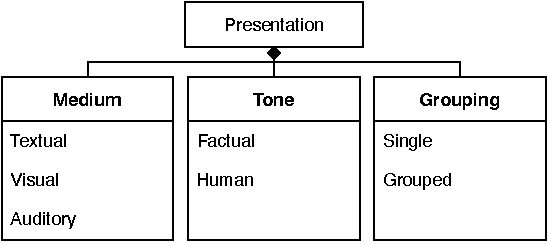
\includegraphics{contents/05_model_description/res/model_presentation_overview.pdf}
    \end{center}
    \caption{Übersicht über die \textit{Presentation} von Erklärungen}
    \label{fig:model_presentation_overview}
\end{figure}

\paragraph{Medium} Das \textit{Medium} einer Erklärung ist der Informationsträger für die \textit{Presentation} der Inhalte. Dabei können verschiedene Möglichkeiten aus dem Multimedia-Bereich verwendet werden. In der Literatur untersucht wurden Texterklärungen (\textit{Textual}), visuelle Darstellungen wie z.B. Diagramme (\textit{Visual}) sowie auditive Erklärungen (\textit{Auditory}). Insbesondere dieser Aspekt bietet Möglichkeiten für Mischformen und Kombinationen \cite{kouki_user_2017}.

\paragraph{Tone} Der \textit{Tone} einer Erklärung bestimmt die Art, wie \textit{End Usern} der Inhalt einer Erklärung näher gebracht wird. Das Spektrum der Möglichkeiten erstreckt sich dabei vor allem zwischen sehr faktisch gehaltenen Erklärungen (\textit{Factual}) und persönlichen bzw. menschlichen Erklärungen (\textit{Human}).

\paragraph{Grouping} Mit dem \textit{Grouping} von Erklärungen wird bestimmt, wie viele Erklärungen \textit{End Usern} gleichzeitig beziehungsweise kombiniert präsentiert werden. Grundsätzlich gibt es dabei die Möglichkeiten eine Erklärung zur Zeit anzuzeigen (\textit{Single}) oder mehrere Erklärungen bzw. Erklärungstypen zu gruppieren (\textit{Grouped}). Bei letzterem können entweder Erklärungen mit verschiedener \textit{Presentation} aber dem gleichen \textit{Content} kombiniert werden \cite{kouki_user_2017} oder mehrere einzelne Erklärungen zusammen dargestellt werden \cite{balog_measuring_2020}.

\bigskip

Als letzter Teil der Antwort auf \textbf{RQ2} kann resultierend die \textit{Presentation} mit den dazugehörigen Aspekten als Eigenschaft von Erklärungen mit einem Einfluss auf die externe Qualität von Erklärungen ergänzt werden.

\newpage

\begin{table}[htb!]
    \begin{center}
        \begin{tabular}{p{.25\textwidth}p{.25\textwidth}p{.41\textwidth}}
            \hline
            Aspekt     & Ausprägung & Quellen \\
            \toprule
            Medium              & Textual  &    \cite{sokol_explainability_2020} \cite{balog_measuring_2020}
                                                \cite{tintarev_designing_nodate} \cite{sato_action-triggering_2019}
                                                \cite{eiband_impact_2019} \cite{eiband_impact_2019}
                                                \cite{abdulrahman_belief-based_2019} \cite{cassens_ambient_2019}
                                                \cite{nunes_systematic_2017} \\
                                & Visual    &   \cite{sokol_explainability_2020} \cite{sato_action-triggering_2019} 
                                                \cite{mucha_interfaces_2021} \cite{abdulrahman_belief-based_2019}
                                                \cite{nunes_systematic_2017} \cite{schrills_color_2020} \\
                                & Auditory     &   \cite{wiegand2019drive} \cite{nunes_systematic_2017}
                                                \cite{wang_is_2018} \\
            \tablerowspacing
            Tone                & Factual   &   \cite{eiband_impact_2019} \cite{abdulrahman_belief-based_2019}
                                                \cite{kunkel_let_2019} \cite{neerincx_using_2018} \\
                                & Human     &   \cite{abdulrahman_belief-based_2019} \cite{kunkel_let_2019}
                                                \cite{weitz_you_2019} \cite{zahedi_towards_2019}
                                                \cite{neerincx_using_2018} \\
            \tablerowspacing
            Grouping            & Single    &   \cite{nunes_systematic_2017} \cite{balog_measuring_2020}
                                                \cite{sato_action-triggering_2019} \cite{eiband_impact_2019}
                                                \cite{abdulrahman_belief-based_2019} \\
                                & Grouped   &   \cite{nunes_systematic_2017} \cite{balog_measuring_2020}
                                                \cite{tintarev_designing_nodate}  \\
            \toprule
        \end{tabular}
    \end{center}
    \caption{Verschiedene Übermittlungsmöglichkeiten für Erklärungen an den \textit{End User}, die in der Literatur einen Effekt auf die externe Qualität von Erklärungen gezeigt haben}
    \label{tab:presentation_of_explanations}
\end{table}

\noindent\fbox{
    \parbox{0.964\textwidth}{
        \smallskip
        \textbf{RQ2} Welche Eigenschaften von Erklärungen haben einen Einfluss auf die externe Qualität eines erklärbaren Systems?
        \smallskip
    }
}

\smallskip

Der in diesem Abschnitt vorgestellte Teil des Modells für Erklärungen (\textit{Characteristics}) beinhaltet die Antwort auf die zweite Forschungsfrage. Dabei sind explizit die Eigenschaften \textit{Demand}, \textit{Content} und \textit{Presentation} mit einem Einfluss auf die externe Qualität von Erklärungen zu benennen. Die genauen Ausprägungen dieser Eigenschaften wurden als Unterpunkte der jeweiligen Aspekte vorgestellt. Die Ergebnisse, die in dem Modell zusammengefasst sind, entspringen dabei der Evaluation von Erklärungen mit verschiedenen Eigenschaften in der Literatur. Der Einfluss auf die externe Qualität ist dabei insofern gewährleistet, als die in dem Modell erwähnten Eigenschaften nur dann Einzug erhalten haben, wenn in mindestens einer wissenschaftlichen Arbeit ein solcher Einfluss festgestellt wurde.